\documentclass[serif,mathserif,final]{beamer}
\mode<presentation>{\usetheme{Whiteboard}}
\usepackage{amsmath,amsfonts,amssymb,pxfonts,eulervm,xspace}
\usepackage{graphicx}
\usepackage[utf8]{inputenc}
\usepackage[brazil]{babel}
\graphicspath{{./figures/}}
\usepackage[orientation=landscape,size=b1,scale=1.0,debug]{beamerposter}

%-- Header and footer information ----------------------------------
% \newcommand{\footleft}{http://github.com/caelum/calopsita}
% \newcommand{\footright}{shawn at shawn lankton dot com}
\newcommand{\calopsita}{Calopsita}
\newcommand{\opensource}{\textit{open source}}

\title{Calopsita: um gerenciador de projetos ágeis}
\author{Alunos: Cauê Haucke Porta Guerra, Cecilia Fernandes, Lucas Cavalcanti dos Santos}
%-------------------------------------------------------------------


%-- Main Document --------------------------------------------------
\begin{document}
\begin{frame}{}
  \begin{columns}[t]

    %-- Text'n info ---------------------------------------------------
    \begin{column}{0.29\linewidth}

      %-- Block 1-1
      \begin{block}{Projetos ágeis}
		Metodologias ágeis têm se mostrado eficazes e é por isso que grandes 
		empresas como Google, IBM, Microsoft adotaram essas práticas de 
		engenharia de \textit{software}. E não apenas as gigantes apostam em 
		\textit{Agile}: por todo o mundo a adoção de metodologias ágeis ganha 
		destaque ano a ano. 
      \end{block}

	  \vspace{1cm}
      
	  %-- Block 1-2
      \begin{block}{Comunicação}
        Ser ágil está intimamente relacionado à comunicação. Clientes e 
		desenvolvedores agem como uma equipe e acompanham de perto o andamento 
		do projeto, as vitórias e as dificuldades.
	
		\vspace{1cm}

		Mas... nada substitui com perfeição um quadro branco e sua efetividade 
		de comunicação. E é cada vez mais comum que trabalhemos, de forma ágil,
		com equipes geograficamente distribuidas. 
      \end{block}

	  \vspace{1cm}
      
      %-- Block 1-3
	  \begin{block}{Calopsita}
		O \textbf{Calopsita} é um sistema \textit{open source} que vem suprir as 
		necessidades das equipes ágeis distribuidas. Ele centraliza as informações, 
		guarda históricos e permite que desenvolvedores e clientes interajam em 
		tempo real.

		\vspace{1pt}

		Mais do que um gerenciador de projetos de Scrum ou XP, o Calopsita se 
		adapta a qualquer metodologia ágil escolhida e às métricas particulares
		de cada projeto, graças à sua arquitetura de plugins.

		\vspace{2cm}
      
		\begin{figure}[htb]
		  \centering
				\fbox{
         	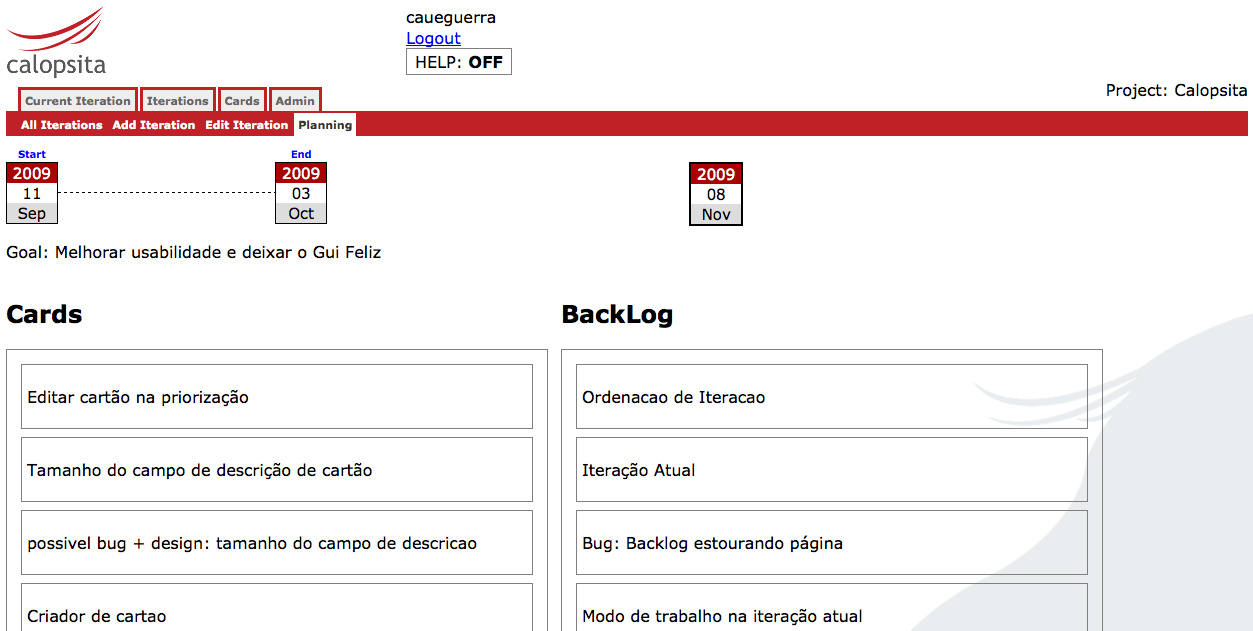
\includegraphics[width=.8\columnwidth]{images/planejamento}
				}
				\caption{Planejamento}
        \end{figure}
				
				\begin{figure}[htb]
         \centering
				\fbox{
         	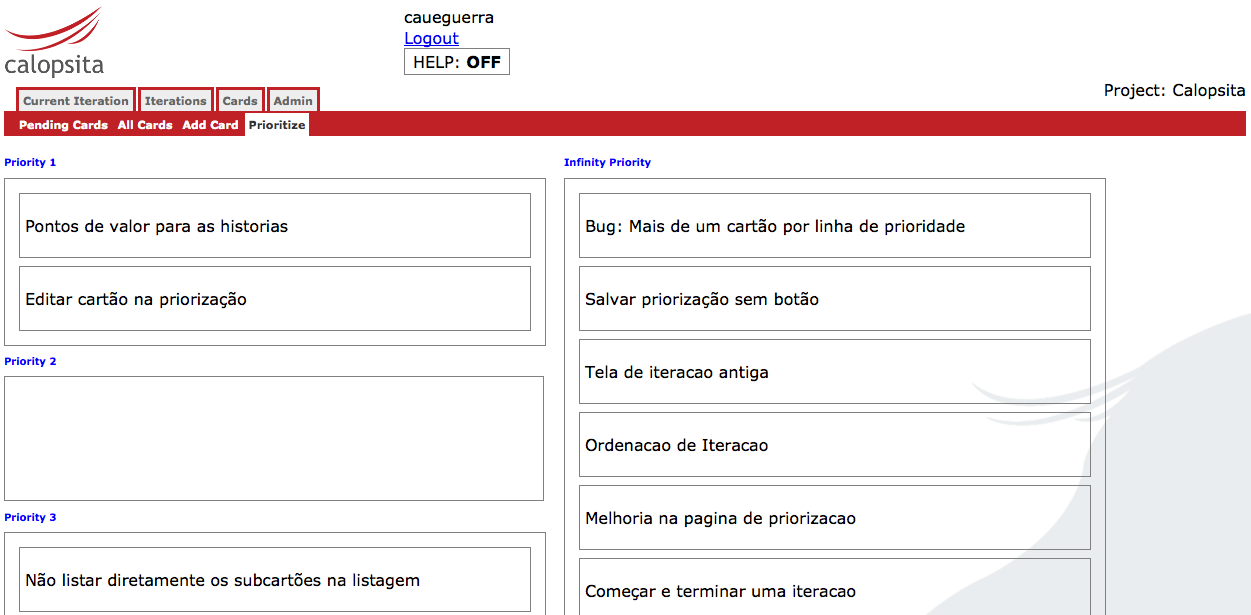
\includegraphics[width=.8\columnwidth]{images/priorizacao}
				}
				\caption{Priorização}
        \end{figure}
      \end{block}

    \end{column} % text'n info

    %-- Whiteboard -------------------------------------------------------
    \begin{column}{0.70\linewidth}

	  \begin{columns}[t] %-- kanban ------------------------------------

		%-- Kanban working -----------------------------------------------
		\begin{column}{0.14\linewidth}

		\end{column}%4

		%-- Kanban todo --------------------------------------------------
		\begin{column}{0.16\linewidth}

		\end{column}% todo

		%-- Kanban working -----------------------------------------------
		\begin{column}{0.16\linewidth}

		\end{column}% working

		%-- Kanban done --------------------------------------------------
		\begin{column}{0.24\linewidth}

		\end{column}% done
	  \end{columns} % kanban

    \end{column}% whiteboard


  \end{columns}
\end{frame}
\end{document}
